%%%%%%%%%%%%%%%%%%%%%%%%%%%%%%%%%%%%%%%%%
% KOMA-Script Presentation
% LaTeX Template
% Version 1.1 (18/10/15)
%
% This template has been downloaded from:
% http://www.LaTeXTemplates.com
%
% Original Authors:
% Marius Hofert (marius.hofert@math.ethz.ch)
% Markus Kohm (komascript@gmx.info)
% Described in the PracTeX Journal, 2010, No. 2
%
% License:
% CC BY-NC-SA 3.0 (http://creativecommons.org/licenses/by-nc-sa/3.0/)
%
%%%%%%%%%%%%%%%%%%%%%%%%%%%%%%%%%%%%%%%%%

%----------------------------------------------------------------------------------------
%	PACKAGES AND OTHER DOCUMENT CONFIGURATIONS
%----------------------------------------------------------------------------------------

\documentclass[
paper=128mm:96mm, % The same paper size as used in the beamer class
fontsize=11pt, % Font size
pagesize, % Write page size to dvi or pdf
parskip=half-, % Paragraphs separated by half a line
]{scrartcl} % KOMA script (article)

\linespread{1.12} % Increase line spacing for readability

%------------------------------------------------
% Colors
\usepackage{xcolor}	 % Required for custom colors
% Define a few colors for making text stand out within the presentation
\definecolor{mygreen}{RGB}{44,85,17}
\definecolor{myblue}{RGB}{34,31,217}
\definecolor{mybrown}{RGB}{194,164,113}
\definecolor{myred}{RGB}{255,66,56}
% Use these colors within the presentation by enclosing text in the commands below
\newcommand*{\mygreen}[1]{\textcolor{mygreen}{#1}}
\newcommand*{\myblue}[1]{\textcolor{myblue}{#1}}
\newcommand*{\mybrown}[1]{\textcolor{mybrown}{#1}}
\newcommand*{\myred}[1]{\textcolor{myred}{#1}}
%------------------------------------------------

%------------------------------------------------
% Margins
\usepackage[ % Page margins settings
includeheadfoot,
top=3.5mm,
bottom=3.5mm,
left=5.5mm,
right=5.5mm,
headsep=6.5mm,
footskip=8.5mm
]{geometry}
%------------------------------------------------

%------------------------------------------------
% Fonts
\usepackage[T1]{fontenc}	 % For correct hyphenation and T1 encoding
\usepackage{lmodern} % Default font: latin modern font
%\usepackage{fourier} % Alternative font: utopia
%\usepackage{charter} % Alternative font: low-resolution roman font
\renewcommand{\familydefault}{\sfdefault} % Sans serif - this may need to be commented to see the alternative fonts
%------------------------------------------------

%------------------------------------------------
% Various required packages
\usepackage{amsthm} % Required for theorem environments
\usepackage{bm} % Required for bold math symbols (used in the footer of the slides)
\usepackage{graphicx} % Required for including images in figures
\usepackage{tikz} % Required for colored boxes
\usepackage{booktabs} % Required for horizontal rules in tables
\usepackage{multicol} % Required for creating multiple columns in slides
\usepackage{lastpage} % For printing the total number of pages at the bottom of each slide
\usepackage[english]{babel} % Document language - required for customizing section titles
\usepackage{microtype} % Better typography
\usepackage{tocstyle} % Required for customizing the table of contents
\usepackage{subcaption}
\usepackage[absolute,overlay]{textpos}
\usepackage{braket} % used for Dirac notation
\usepackage{amsmath} %used for gather
\usepackage{amsfonts}
\usepackage{algorithmicx}
\usepackage{algpseudocode} % together for code

\makeatletter
\algrenewcommand\ALG@beginalgorithmic{\tiny}
\makeatletter

%------------------------------------------------

%------------------------------------------------
% Slide layout configuration
\usepackage{scrpage2} % Required for customization of the header and footer
\pagestyle{scrheadings} % Activates the pagestyle from scrpage2 for custom headers and footers
\clearscrheadfoot % Remove the default header and footer
\setkomafont{pageheadfoot}{\normalfont\color{black}\sffamily} % Font settings for the header and footer

% Sets vertical centering of slide contents with increased space between paragraphs/lists
\makeatletter
\renewcommand*{\@textbottom}{\vskip \z@ \@plus 1fil}
\newcommand*{\@texttop}{\vskip \z@ \@plus .5fil}
\addtolength{\parskip}{\z@\@plus .25fil}
\makeatother

% Remove page numbers and the dots leading to them from the outline slide
\makeatletter
\newtocstyle[noonewithdot]{nodotnopagenumber}{\settocfeature{pagenumberbox}{\@gobble}}
\makeatother
\usetocstyle{nodotnopagenumber}

\AtBeginDocument{\renewcaptionname{english}{\contentsname}{\Large Outline}} % Change the name of the table of contents
%------------------------------------------------

%------------------------------------------------
% Header configuration - if you don't want a header remove this block
\newcommand\myhead[1]{\ihead{
\hspace{-2mm}
\begin{tikzpicture}[remember picture,overlay]
\node [xshift=\paperwidth/2,yshift=-\headheight] (mybar) at (current page.north west)[rectangle,fill,inner sep=0pt,minimum width=\paperwidth,minimum height=2\headheight,top color=mygreen!64,bottom color=mygreen]{}; % Colored bar
\node[below of=mybar,yshift=3.3mm,rectangle,shade,inner sep=0pt,minimum width=128mm,minimum height =1.5mm,top color=black!50,bottom color=white]{}; % Shadow under the colored bar
shadow
\end{tikzpicture}
\color{white}#1}} % Header text defined by the \runninghead command below and colored white for contrast
%------------------------------------------------ 

%------------------------------------------------
% Footer configuration
\setlength{\footheight}{8mm} % Height of the footer
\addtokomafont{pagefoot}{\footnotesize} % Small font size for the footnote

\ifoot{% Left side
\hspace{-2mm}
\begin{tikzpicture}[remember picture,overlay]
\node [xshift=\paperwidth/2,yshift=\footheight] at (current page.south west)[rectangle,fill,inner sep=0pt,minimum width=\paperwidth,minimum height=3pt,top color=mygreen,bottom color=mygreen]{}; % Green bar
\end{tikzpicture}
\myauthor\ \raisebox{0.2mm}{$\bm{\vert}$}\ \myuni % Left side text
}

\ofoot[\pagemark/\pageref{LastPage}\hspace{-2mm}]{\pagemark/\pageref{LastPage}\hspace{-2mm}} % Right side
%------------------------------------------------

%------------------------------------------------
% Section spacing - deeper section titles are given less space due to lesser importance
\usepackage{titlesec} % Required for customizing section spacing
\titlespacing{\section}{0mm}{0mm}{0mm} % Lengths are: left, before, after
\titlespacing{\subsection}{0mm}{0mm}{-1mm} % Lengths are: left, before, after
\titlespacing{\subsubsection}{0mm}{0mm}{-2mm} % Lengths are: left, before, after
\setcounter{secnumdepth}{0} % How deep sections are numbered, set to no numbering by default - change to 1 for numbering sections, 2 for numbering sections and subsections, etc
%------------------------------------------------

%------------------------------------------------
% Theorem style
\newtheoremstyle{mythmstyle} % Defines a new theorem style used in this template
{0.5em} % Space above
{0.5em} % Space below
{} % Body font
{} % Indent amount
{\sffamily\bfseries} % Head font
{} % Punctuation after head
{\newline} % Space after head
{\thmname{#1}\ \thmnote{(#3)}} % Head spec
	
\theoremstyle{mythmstyle} % Change the default style of the theorem to the one defined above
\newtheorem{theorem}{Theorem}[section] % Label for theorems
\newtheorem{remark}[theorem]{Remark} % Label for remarks
\newtheorem{algorithm}[theorem]{Algorithm} % Label for algorithms
\makeatletter % Correct qed adjustment
%------------------------------------------------

%------------------------------------------------
% The code for the box which can be used to highlight an element of a slide (such as a theorem)
\newcommand*{\mybox}[2]{ % The box takes two arguments: width and content
\par\noindent
\begin{tikzpicture}[mynodestyle/.style={rectangle,draw=mygreen,thick,inner sep=2mm,text justified,top color=white,bottom color=white,above}]\node[mynodestyle,at={(0.5*#1+2mm+0.4pt,0)}]{ % Box formatting
\begin{minipage}[t]{#1}
#2
\end{minipage}
};
\end{tikzpicture}
\par\vspace{-1.3em}}
%------------------------------------------------

%----------------------------------------------------------------------------------------
%	PRESENTATION INFORMATION
%----------------------------------------------------------------------------------------

\newcommand*{\mytitle}{Infinite Matter Calculations} % Title
\newcommand*{\mysubtitle}{Coupled Cluster Doubles} %Subtitle
\newcommand*{\runninghead}{Running Head} % Running head displayed on almost all slides
\newcommand*{\myauthor}{Sam Novario, Justin Lietz} % Presenters name(s)
\newcommand*{\mydate}{\today} % Presentation date
\newcommand*{\myuni}{Michigan State University --- NSCL} % University or department

%----------------------------------------------------------------------------------------

\begin{document}

%----------------------------------------------------------------------------------------
%	TITLE SLIDE
%----------------------------------------------------------------------------------------

% Title slide - you may have to tweak a few of the numbers if you wish to make changes to the layout
\thispagestyle{empty} % No slide header and footer
\begin{tikzpicture}[remember picture,overlay] % Background box
\node [xshift=\paperwidth/2,yshift=\paperheight/2] at (current page.south west)[rectangle,fill,inner sep=0pt,minimum width=\paperwidth,minimum height=\paperheight/2,top color=mygreen,bottom color=mygreen]{}; % Change the height of the box, its colors and position on the page here
\end{tikzpicture}
% Text within the box
\begin{flushright}
\vspace{0.4cm}
\color{white}\sffamily
{\bfseries\Large\mytitle\par} % Title
{\bfseries\mysubtitle\par} % Subtitle
\vspace{0.5cm}
\normalsize
\myauthor\par % Author name
\mydate\par % Date
\vfill
\end{flushright}

\clearpage

%----------------------------------------------------------------------------------------
%	PRESENTATION SLIDES
%----------------------------------------------------------------------------------------

\myhead{Infinite-Matter Basis}
\centering
Free-Particle Hamiltonian,
\begin{equation*}
\frac{-\hbar^2}{2m}\nabla^2\mathop{\phi(\vec{x})}=\epsilon\mathop{\phi(\vec{x})}.
\end{equation*}
Periodic Boundary Conditions in L-Box
\begin{gather*}
\mathop{\phi(x,y,z)}=\mathop{\phi(x+L,y,z)} \\
\mathop{\phi(x,y,z)}=\mathop{\phi(x,y+L,z)} \\
\mathop{\phi(x,y,z)}=\mathop{\phi(x,y,z+L)}
\end{gather*}
Single-Particle States
\begin{equation*}
\mathop{\phi_{\vec{k}}(\vec{x})}=\frac{1}{\sqrt{L^{3}}}e^{i\vec{k}\cdot\vec{x}},\hspace{0.5cm}\vec{k}=\frac{2\pi\vec{n}}{L},\hspace{0.5cm}n_{i}\in\mathbb{I}
\end{equation*}

\clearpage

\centering
\begin{minipage}{7cm}
  \vspace{-0.4cm}
  \begin{equation*}
    \text{Energy Truncation: }n_{x}^{2}+n_{x}^{2}+n_{x}^{2}\leq N_{\text{max}}
  \end{equation*}
  \vspace{-0.75cm}
  \begin{algorithmic}
    \State $n=0$
    \For{$\text{shell}\in\{ 0,...,N_{\text{max}}\}$}
    \For{$\sqrt{N_{\text{max}}}\leq n_{x}\leq\sqrt{N_{\text{max}}}$}
    \For{$\sqrt{N_{\text{max}}}\leq n_{y}\leq\sqrt{N_{\text{max}}}$}
    \For{$\sqrt{N_{\text{max}}}\leq n_{z}\leq\sqrt{N_{\text{max}}}$}
    \For{$s_{z}\in\{-\frac{1}{2},\frac{1}{2}\}$}
    \If{$n_{x}^{2}+n_{y}^{2}+n_{z}^{2}=\text{shell}$}
    \State $\text{Energy}=\frac{4\pi^{2}\hbar^{2}}{2m}\times\text{shell}$
    \If{$n<N$}
    \State $\text{type}=\text{``hole''}$
    \Else
    \State $\text{type}=\text{``particle''}$
    \EndIf
    \State STATES $\gets$ ($n$, $n_{x}$, $n_{y}$, $n_{z}$, $s_{z}$, Energy, type)
    \State $n\gets n+1$
    \EndIf
    \EndFor
    \EndFor
    \EndFor
    \EndFor
    \EndFor
  \end{algorithmic}
\end{minipage}

\clearpage

%-----------------------------------------------

\myhead{Two-Body Channels}
\centering
\begin{minipage}{8cm}
  \vspace{-0.5cm}
  \begin{gather*}
    \braket{pq||rs}\Rightarrow\braket{\mathop{T(pq)}||\mathop{T(rs)}} \\
    \braket{pq||rs}=\braket{ps^{-1}||rq^{-1}}\Rightarrow\braket{\mathop{X(ps)}||\mathop{X(rq)}}
  \end{gather*}
  \centering
  \begin{minipage}{6cm}
    \vspace{0.25cm}
    \begin{algorithmic}
      \For{$\text{sp1}\in STATES$}
      \For{$\text{sp2}\in STATES$}
      \If{$sp1\neq sp2$}
      \State $N_{i}\gets n_{i,1}+n_{i,2}$
      \State $S_{z}\gets s_{z,1}+s_{z,2}$
      \State $T_{z}\gets t_{z,1}+t_{z,2}$
      \State $\text{i\_dir}\gets\text{Ind}\left(N_{x},N_{y},N_{z},S_{z},T_{z}\right)$
      \State $T\gets$ (sp1, sp2, i\_dir)
      \State $N'_{i}\gets n_{i,1}-n_{i,2}$
      \State $S'_{z}\gets s_{z,1}-s_{z,2}$
      \State $T'_{z}\gets t_{z,1}-t_{z,2}$
      \State $\text{i\_cross}\gets\text{Ind}\left(N'_{x},N'_{y},N'_{z},S'_{z},T'_{z}\right)$
      \State $X\gets$ (sp1, sp2, i\_cross)
      \EndIf
      \EndFor
      \EndFor
    \end{algorithmic}
  \end{minipage}
\end{minipage}

\clearpage

%-----------------------------------------------

\myhead{One,Three-Body Channels}
\centering
\begin{minipage}{8cm}
  \vspace{0.5cm}
  \begin{gather*}
    \braket{pq||rs}=\braket{p||q^{-1}rs}\Rightarrow\braket{\mathop{K(p)}||\mathop{K_{p}(qrs)}}
  \end{gather*}
  \centering
  \begin{minipage}{5cm}
    \vspace{0.5cm}
    \begin{algorithmic}
      \For{$\text{Chan}\in T$}
      \For{$\text{tb1}\in\text{Chan}$}
      \For{$\text{tb2}\in\text{Chan}$}
      \State $K\gets\text{tb1}_{1}$
      \State $K_{\text{tb1}_{1}}\gets\mathop{\text{tb1}_{2},\text{tb2}_{1},\text{tb2}_{2}}$
      \EndFor
      \EndFor
      \EndFor
    \end{algorithmic}
  \end{minipage}
\end{minipage}

\clearpage

%-----------------------------------------------

\myhead{CCD Equations}
\begin{gather*}
t_{ij}^{ab}\epsilon^{ab}_{ij} = \braket{ab|\hat{v}|ij} + \frac{1}{2}\sum_{cd}\braket{ab|\hat{v}|cd} t_{ij}^{cd} + \frac{1}{2}\sum_{kl}\braket{kl|\hat{v}|ij} t_{kl}^{ab} \\
+ \mathop{\hat{P}(ij|ab)}\sum_{kc}\braket{kb|\hat{v}|cj}t_{ik}^{ac} + \frac{1}{4}\sum_{klcd}\braket{kl|\hat{v}|cd}t_{ij}^{cd}t_{kl}^{ab} \\
+ \mathop{\hat{P}(ij)}\sum_{klcd}\braket{kl|\hat{v}|cd}t_{ik}^{ac}t_{jl}^{bd} - \frac{1}{2}\mathop{\hat{P}(ij)}\sum_{klcd}\braket{kl|\hat{v}|cd}t_{ik}^{dc}t_{lj}^{ab} \\
- \frac{1}{2}\mathop{\hat{P}(ab)}\sum_{klcd}\braket{kl|\hat{v}|cd}t_{lk}^{ac}t_{ij}^{db}
\end{gather*}

\clearpage

%-----------------------------------------------

\myhead{CCD Intermediates}
\begin{gather*}
\braket{b| \chi |c} = \braket{b|f|c} - \frac{1}{2} \sum_{kld} \braket{bd|t|kl} \braket{kl|v|cd} \\
\braket{k| \chi |j} = \braket{k|f|j} + \frac{1}{2} \sum_{cdl} \braket{kl|v|cd} \braket{cd|t|jl} \\ 
\braket{kl| \chi |ij} = \braket{kl|v|ij} + \frac{1}{2} \sum_{cd} \braket{kl|v|cd} \braket{cd|t|ij} \\
\braket{kb| \chi |cj} = \braket{kb|v|cj} + \frac{1}{2} \sum_{dl} \braket{kl|v|cd} \braket{db|t|lj} \\
\braket{ab| \chi |cd} = \braket{ab|v|cd} 
\end{gather*}

\clearpage

%-----------------------------------------------

\myhead{CCD Equations with Intermediates}
\begin{gather*}
t_{ij}^{ab}\epsilon^{ab}_{ij} = \braket{ab|\hat{v}|ij} + \mathop{\hat{P}(ab)}\sum_{c}\braket{b|\chi|c}t_{ij}^{ac} - \mathop{\hat{P}(ij)}\sum_{k}\braket{k|\chi|j}t_{ik}^{ab} \\ 
+ \frac{1}{2}\sum_{cd}\braket{ab|\chi|cd}t_{ij}^{cd} + \frac{1}{2}\sum_{kl}\braket{kl|\chi|ij}t_{kl}^{ab} \\ 
+ \mathop{\hat{P}(ij|ab)}\sum_{kc}\braket{kb|\chi|cj}t_{ik}^{ac}
\end{gather*}

\clearpage

%-----------------------------------------------

\myhead{Intermediates as Matrix-Matrix Multiplications}
\begin{gather*}
\braket{b|\chi|c} \Rightarrow f_{c}^{b}\mathop{(K(b),K(c))} - \frac{1}{2}t_{kl}^{bd}\mathop{(K(b),K_{b}(kld))}\cdot v_{cd}^{kl}\mathop{(K_{c}(kld),K(c))} \\
\braket{k|\chi|j} \Rightarrow f_{j}^{k}\mathop{(K(k),K(j))} + \frac{1}{2}v_{cd}^{kl}\mathop{(K(k),K_{k}(cdl))}\cdot t_{jl}^{cd}\mathop{(K_{j}(cdl),K(j))} \\
\braket{kl|\chi|ij} \Rightarrow v_{ij}^{kl}\mathop{(T(kl),T(ij))} + \frac{1}{2}v_{cd}^{kl}\mathop{(T(kl),T(cd))}\cdot t_{ij}^{cd}\mathop{(T(cd),T(ij))} \\
\braket{kb|\chi|cj} \Rightarrow v_{cj}^{kb}\mathop{(X(kc),X(jb))} + \frac{1}{2}v_{cd}^{kl}\mathop{(X(kc),X(dl))}\cdot t_{lj}^{db}\mathop{(X(dl),X(jb))} \\
\braket{ab|\chi|cd} \Rightarrow v_{cd}^{ab}\mathop{(T(ab),T(cd))}
\end{gather*}

\clearpage

%----------------------------------------------

\myhead{CCD Equations as Matrix-Matrix Multiplications}
\begin{gather*}
\sum_{c}\braket{b|\chi|c}\braket{ac|t|ij} \Rightarrow \chi_{c}^{b}\mathop{(K(b),K(c))}\cdot t_{ij}^{ac}\mathop{(K(c),K_{c}(ija))} \\
\sum_{k}\braket{k|\chi|j}\braket{ab|t|ik} \Rightarrow \chi_{j}^{k}\mathop{(K(j),K(k))}\cdot t_{ik}^{ab}\mathop{(K(c),K_{c}(ija))} \\
\sum_{cd}\braket{ab|\chi|cd}\braket{cd|t|ij} \Rightarrow \chi_{cd}^{ab}\mathop{(T(ab),T(cd))}\cdot t_{ij}^{cd}\mathop{(T(cd),T(ij))} \\
\sum_{kl}\braket{ab|t|kl}\braket{kl|\chi|ij} \Rightarrow t_{kl}^{ab}\mathop{(T(ab),T(kl))}\cdot \chi_{ij}^{kl}\mathop{(T(kl),T(ij))} \\ 
\sum_{kc}\braket{ac|t|ik}\braket{kb|\chi|cj} \Rightarrow t_{ik}^{ac}\mathop{(X(ia),X(kc))}\cdot \chi_{cj}^{kb}\mathop{(X(kc),X(jb))}
\end{gather*}

\clearpage

%-----------------------------------------------

\myhead{Minnesota Potential}
\begin{minipage}{10cm}
  \vspace{-0.3cm}
  \begin{gather*}
    \mathop{V(r)}=\frac{1}{2}\mathop{(V_{R}+\frac{1}{2}\mathop{(1+P_{12}^{\sigma})}V_{T}+\frac{1}{2}\mathop{(1-P_{12}^{\sigma})} V_{S})}\mathop{(1-P_{12}^{\sigma}P_{12}^{\tau})}, \\
    V_{\alpha}\left( r\right)=V_{\alpha}e^{-\kappa_{\alpha} r^{2}},\ P_{12}^{\sigma}=\frac{1}{2}\mathop{(1+\sigma_{1}\cdot\sigma_{2})},\ P_{12}^{\tau}=\frac{1}{2}\mathop{(1+\tau_{1}\cdot\tau_{2})} 
  \end{gather*}
  \begin{center}
    \begin{tabular}{| l | l | l |}
      \hline
      $\alpha$ & $V_{\alpha}$ & $\kappa_{\alpha}$ \\ \hline
      $R$ & 200 $\mathrm{MeV}$ & 1.487 $\mathrm{fm}^{-2}$ \\ \hline
      $T$ & 178 $\mathrm{MeV}$ & 0.639 $\mathrm{fm}^{-2}$ \\ \hline
      $S$ & 91.85 $\mathrm{MeV}$ & 0.465 $\mathrm{fm}^{-2}$ \\ \hline
    \end{tabular}
  \end{center}
  \vspace{-0.25cm}
  \begin{gather*}
    \braket{pq| V_{\alpha} |rs}=\frac{V_{\alpha}}{L^{3}}\left(\frac{\pi}{\alpha}\right)^{3/2}e^{\frac{-q^{2}}{4\alpha}}\delta_{\vec{k}_{p}+\vec{k}_{q},\vec{k}_{r}+\vec{k}_{s}} \\
    \vec{q}=\frac{1}{2}\left(\vec{k}_{p}-\vec{k}_{q}-\vec{k}_{r}+\vec{k}_{s}\right)
  \end{gather*}
\end{minipage}

\clearpage

%-----------------------------------------------

\myhead{Pure Neutron Matter}
\begin{figure}[!ht]
\centering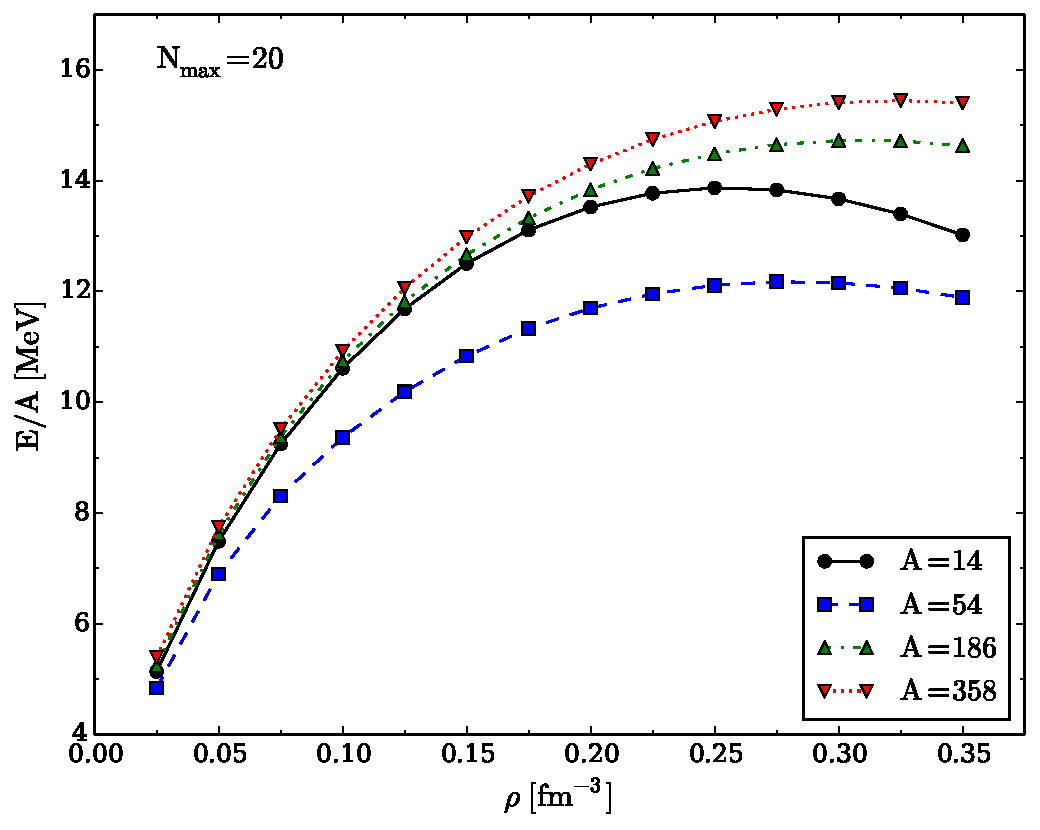
\includegraphics[width=0.7\linewidth]{fig1}
\end{figure}

\clearpage

%------------------------------------------------

\myhead{Pure Neutron Matter}
\begin{figure}[!ht]
\centering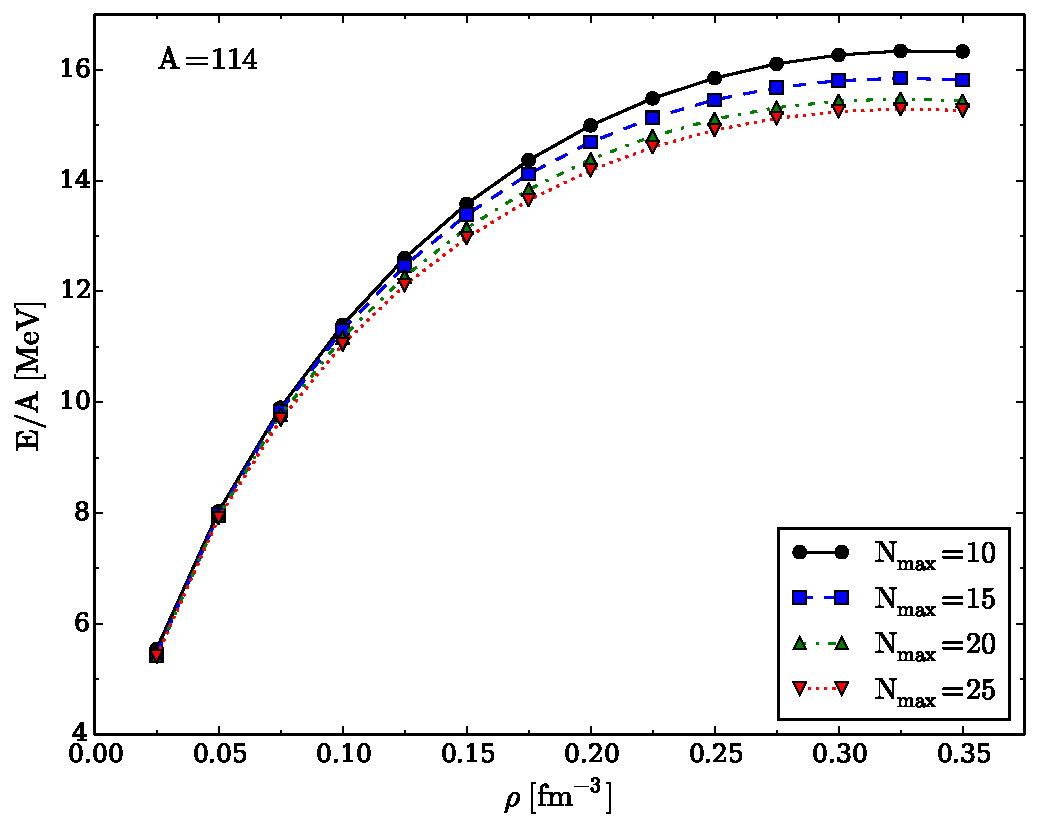
\includegraphics[width=0.7\linewidth]{fig2}
\end{figure}

\clearpage

%------------------------------------------------

\myhead{Twist Averaging}
\begin{equation*}
\mathop{\phi_{\vec{k}}(\vec{x}+\vec{L})}\rightarrow\mathop{e^{i\vec{\theta}}\phi_{\vec{k}}(\vec{x})}
\end{equation*}
$\theta_{i}=0$ for PBC and $\theta_{i}=\pi$ for APBC
\begin{gather*}
\vec{k}\rightarrow\vec{k}+\frac{\vec{\theta}}{L} \\
\epsilon_{\vec{k}}\rightarrow\epsilon_{\vec{k}}+\frac{\pi}{L}\vec{k}\cdot\vec{\theta}+\frac{\pi^{2}}{L^{2}}
\end{gather*}

\clearpage

%------------------------------------------------

\myhead{Twist Averaging}
\centering
\begin{minipage}{10cm}
  \vspace{0.5cm}
  Build Gauss-Legendre Mesh for Each Direction, $\mathop{\{\theta_{i},w_{i}\}}$
  \centering
  \begin{minipage}{6cm}
    \vspace{0.5cm}
    \begin{algorithmic}
      \State $E_{\text{twist}}=0$
      \For{$\mathop{(\theta_{x},w_{x})}\in\mathop{\{\theta_{x},w_{x}\}}$}
      \For{$\mathop{(\theta_{y},w_{y})}\in\mathop{\{\theta_{y},w_{y}\}}$}
      \For{$\mathop{(\theta_{z},w_{z})}\in\mathop{\{\theta_{z},w_{z}\}}$}
      \State Build Basis States with $k_{i}\rightarrow k_{i}+\frac{\theta_{i}}{L}$
      \State Order States by Energy and Fill Holes
      \State Get Result $E$ (T,HF,CCD)
      \State $E_{\text{twist}}=E_{\text{twist}}+\frac{1}{\pi^{3}}w_{x}w_{y}w_{z}E$
      \EndFor
      \EndFor
      \EndFor
    \end{algorithmic}
  \end{minipage}
\end{minipage}

\clearpage

%-----------------------------------------------

\myhead{Pure Neutron Matter - Twist Averaging}
$\text{T}_{\text{inf}}=\frac{3\hbar^{2}k_{f}^{2}}{10m}$
\begin{figure}[!ht]
  \centering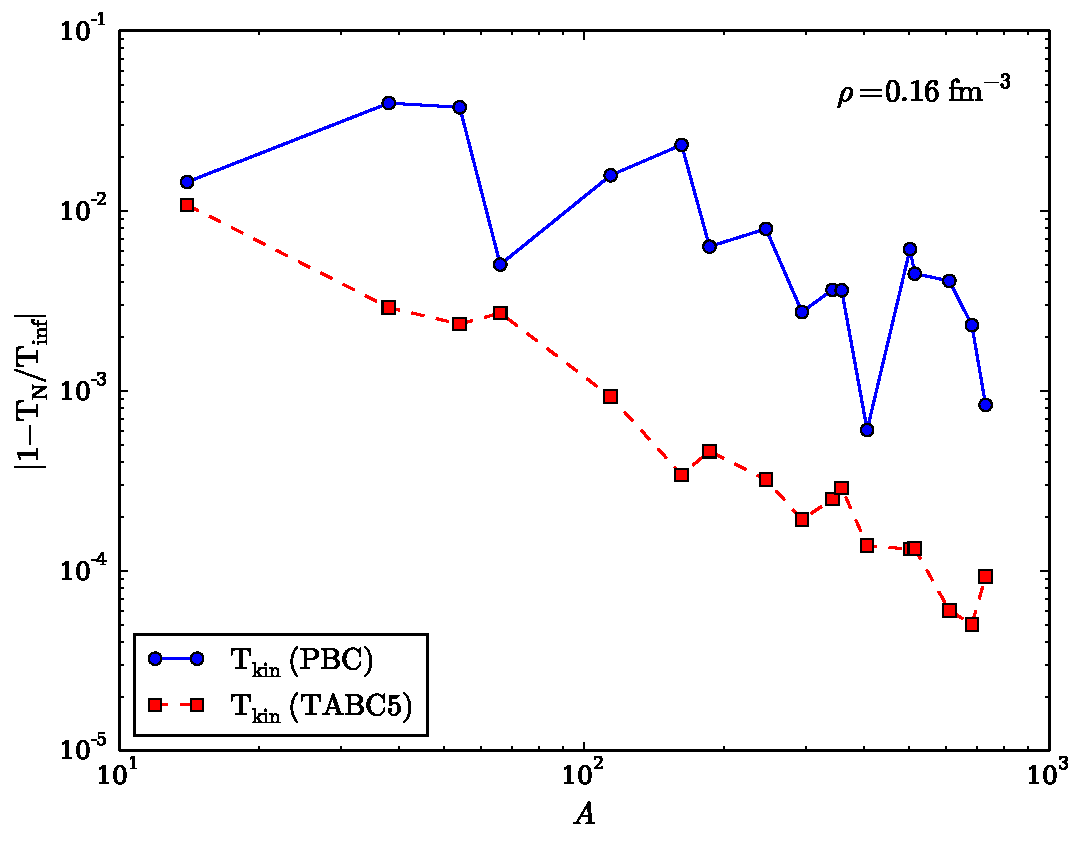
\includegraphics[width=0.6\linewidth]{fig3}
\end{figure}

\clearpage

%------------------------------------------------

\myhead{Pure Neutron Matter - Twist Averaging}
$\text{HF}_{\text{inf}}=\frac{1}{\mathop{(2\pi)^{6}}}\frac{L^{3}}{2\rho}\int_{0}^{k_{f}}d\vec{k}_{1}\int_{0}^{k_{f}}d\vec{k}_{2}\braket{\vec{k}_{1}\vec{k}_{2}|\hat{v}|\vec{k}_{1}\vec{k}_{2}}$
\begin{figure}[!ht]
\centering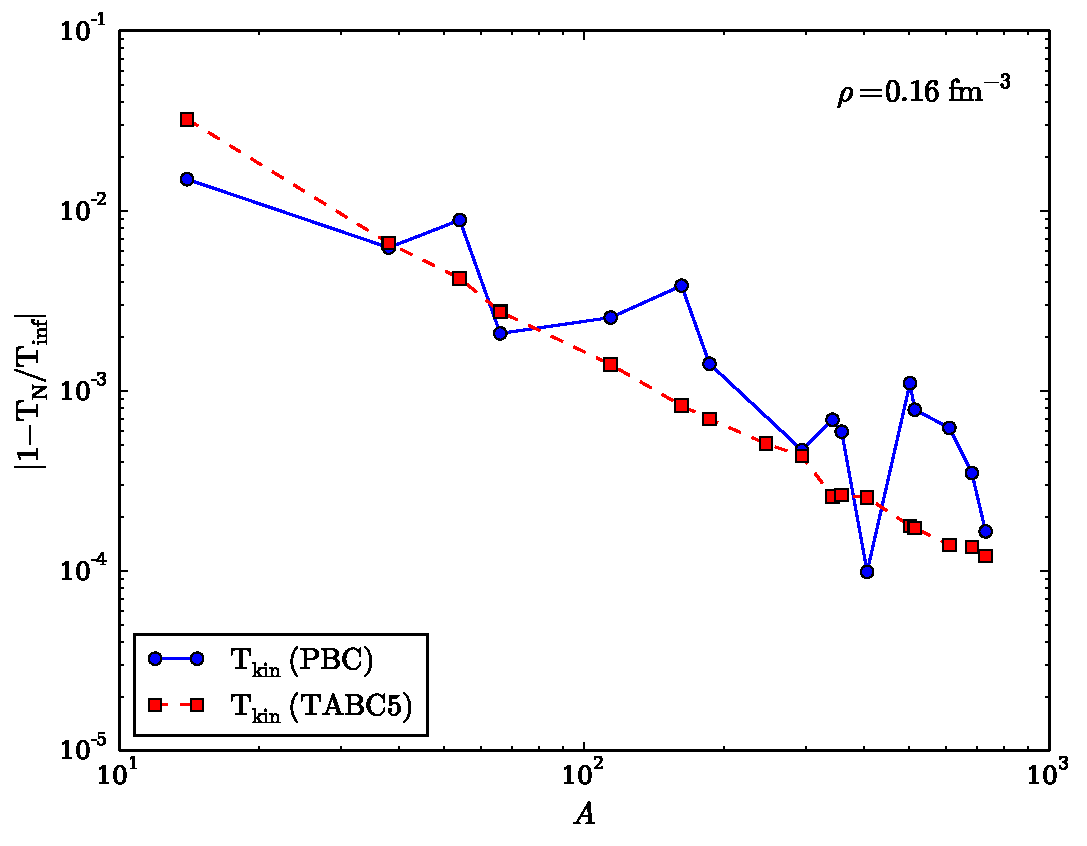
\includegraphics[width=0.6\linewidth]{fig4}
\end{figure}

\clearpage

%------------------------------------------------

\end{document}
